\chapter{Control Flow Graph}
\label{ch:cfg}

A Control Flow Graph (CFG) is a graphical representation of the control flow or flow of execution within a program. It illustrates how the program's instructions or statements are connected and executed based on various control structures such as conditionals (if-else statements), loops (for, while statements), and function calls.

In a CFG, each node represents a basic block, which is a sequence of instructions with a single entry point and a single exit point. The nodes are connected by directed edges that represent the flow of control between the basic blocks. The edges indicate the order in which the basic blocks are executed. Figure \ref{fig:cfg_numbers} presents an example of CFG.

\begin{figure}[!ht]
    \centering
    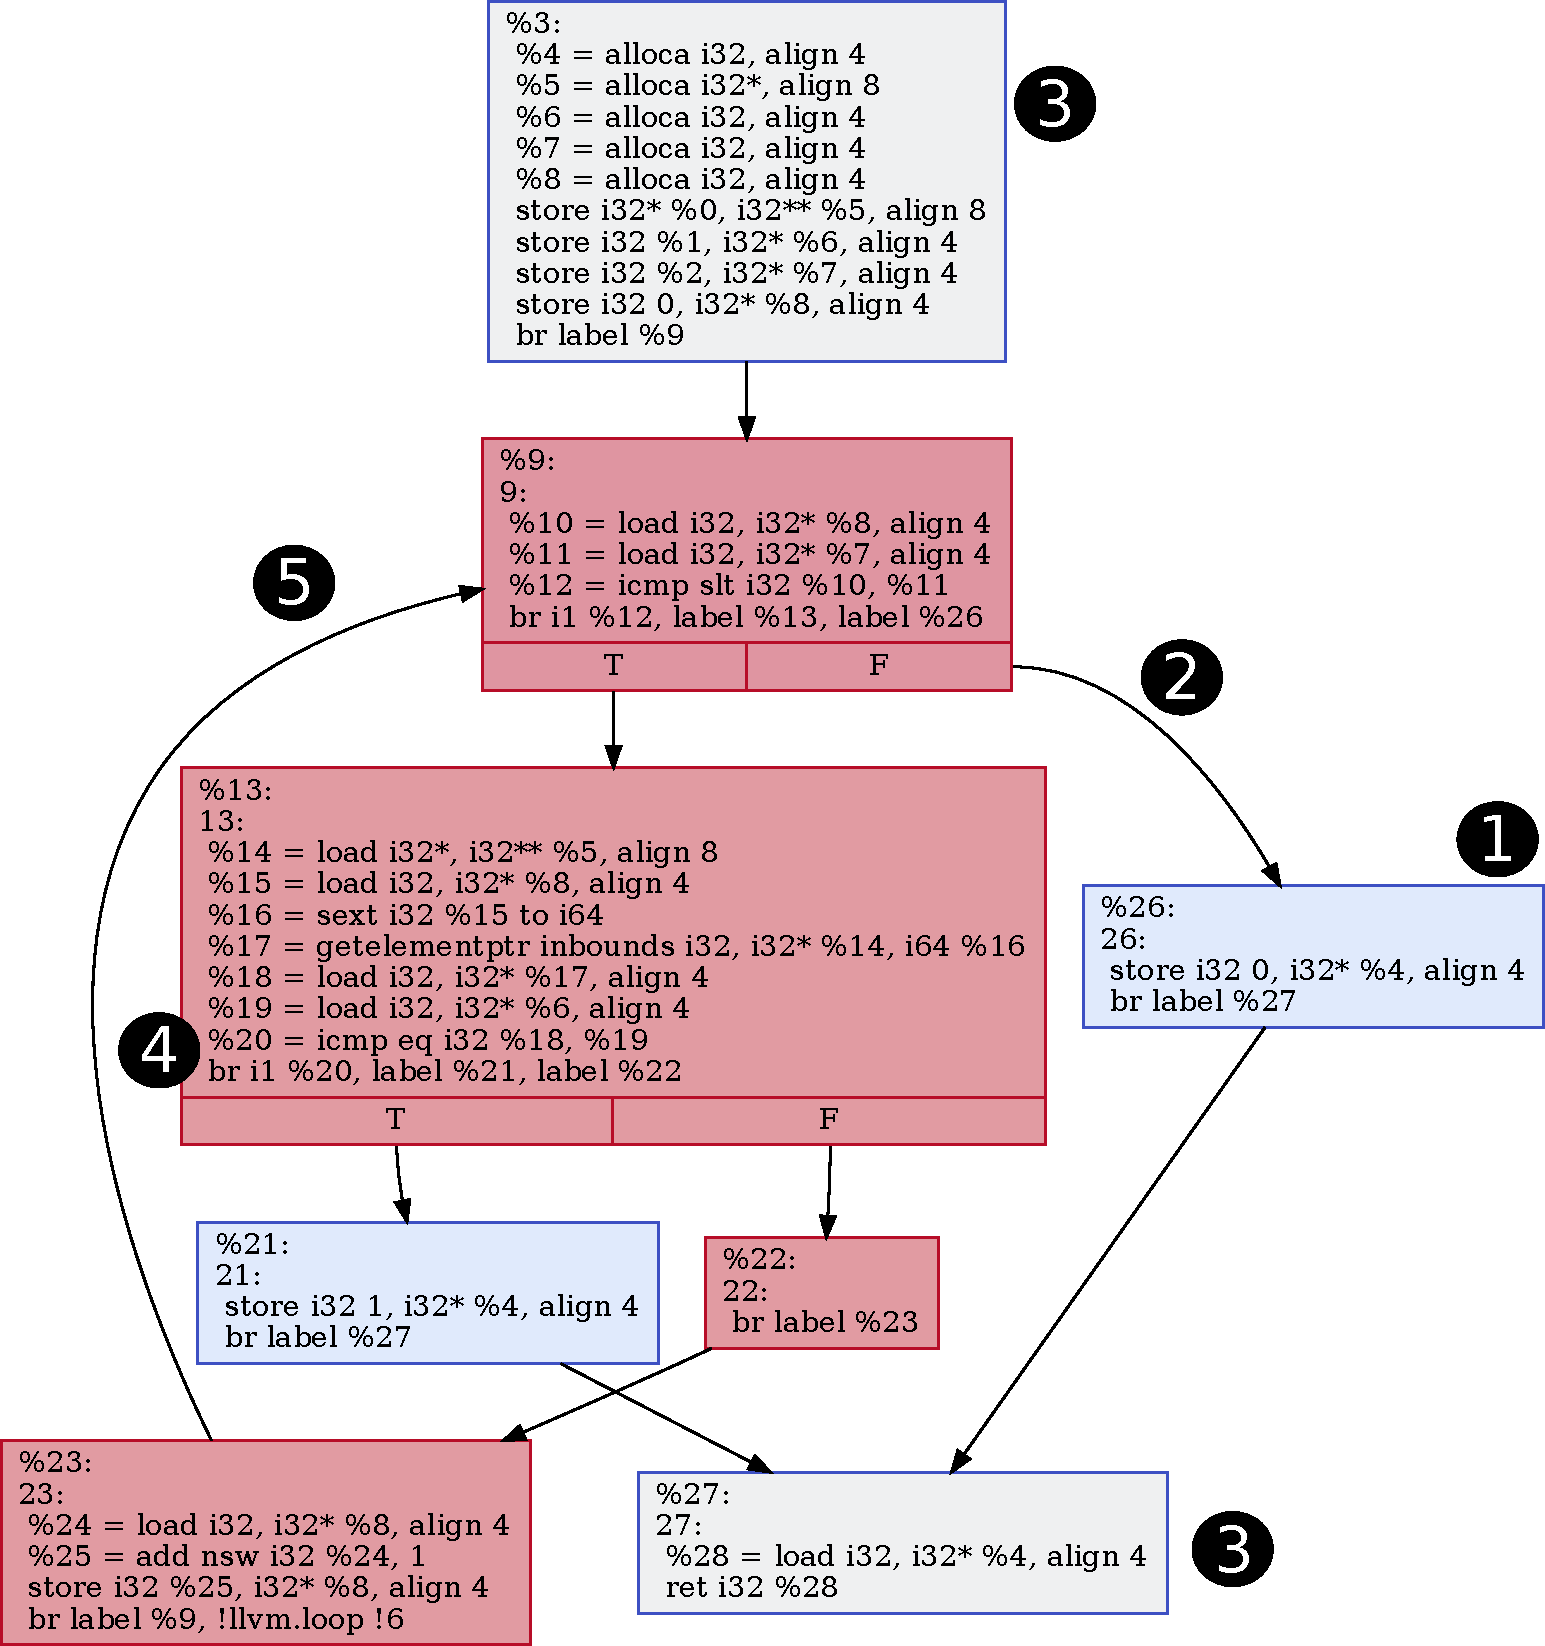
\includegraphics[width=0.95\textwidth]{images/cfg_numbers.pdf}
    \caption{CFG's example}
    \label{fig:cfg_numbers}
\end{figure}

The key components of a Control Flow Graph are: 

\begin{enumerate}
    \item \textbf{Nodes/Basic Blocks:} Each node in the CFG represents a basic block, which is a sequence of instructions with a single entry point and a single exit point. A basic block typically consists of a straight-line sequence of instructions without any branches.
    \item \textbf{Edges:} The edges in the CFG represent the flow of control between the basic blocks. They show how the program transitions from one basic block to another based on the execution of statements such as conditionals, loops, or function calls.
    \item \textbf{Entry and Exit Nodes:} The entry node represents the starting point of the program, and the exit node represents the endpoint or termination of the program. These nodes are connected to the rest of the CFG and provide the overall structure of the control flow.
    \item \textbf{Branching Statements:} Conditional statements, such as if-else or switch statements, introduce branches in the control flow. Branches create multiple paths in the CFG, leading to different basic blocks depending on the evaluated conditions.
    \item \textbf{Loops:} Loop statements, such as for or while loops, introduce repetitive execution in the control flow. The CFG represents loops by creating back edges that connect the exit point of the loop to the entry point, allowing the loop to iterate until the exit condition is met.
\end{enumerate}

CFGs are commonly used in program analysis, optimization, and debugging. They provide a visual representation of the program's control flow, enabling developers and researchers to analyze the program's behavior, identify potential issues, understand code coverage, and perform optimizations or transformations on the program's control flow structure. CFGs are particularly useful for understanding complex programs with multiple control structures and decision points.

\subsection{Generating CFGs with LLVM}

LLVM provides a powerful infrastructure for generating Control Flow Graphs (CFGs) for programs. The LLVM framework, along with its intermediate representation (IR) and associated tools, can be used to analyze and visualize the control flow of code.

The code which we will use as an example will be this:

\begin{lstlisting}[language=C++]
void foo(int** a, int N) {
    int i, j;
    for (i = 0; i < N; i++) {
        for (j = 0; j < N; j++) {
            a[i][j] = 0;
        }
    }
    for (i = 0; i < N; i++) {
        a[i][i] = 1;
    }
}
\end{lstlisting}

First, you need to compile your source code to LLVM IR using the LLVM compiler, such as Clang. Clang can generate LLVM IR from various programming languages like C, C++, and Swift. Use the appropriate compiler flags to emit the LLVM IR instead of generating object files or executables. Example:

\begin{verbatim}
    $ clang -Xclang -disable-O0-optnone -S -emit-llvm foo.c -o foo.ll
\end{verbatim}

Once you have the LLVM IR file, you can use LLVM's API or tools to load and manipulate the IR. The LLVM C++ API provides rich functionality for working with IR, and various command-line tools like \textbf{llvm-dis}, \textbf{llvm-as}, or \textbf{opt} can be used to process the IR. We will use the opt command:

\begin{verbatim}
    $ opt -dot-cfg foo.ll -disable-output
\end{verbatim}

Once you have built the CFG, you can either visualize it graphically or perform further analysis or transformations. There are various graph visualization tools available, such as Graphviz or the LLVM dot tool, which can generate graphical representations of the CFG.

Example command to generate a graphical CFG using LLVM's dot tool:

\begin{verbatim}
    $ dot -Tpdf .foo.dot -o foo.pdf
\end{verbatim}

In the end, the result is shown in Figure \ref{fig:cfg_foo}. Remember to refer to the LLVM documentation, tutorials, and examples for more detailed information on using the LLVM APIs and tools to generate and work with CFGs.

\begin{figure}[!ht]
    \centering
    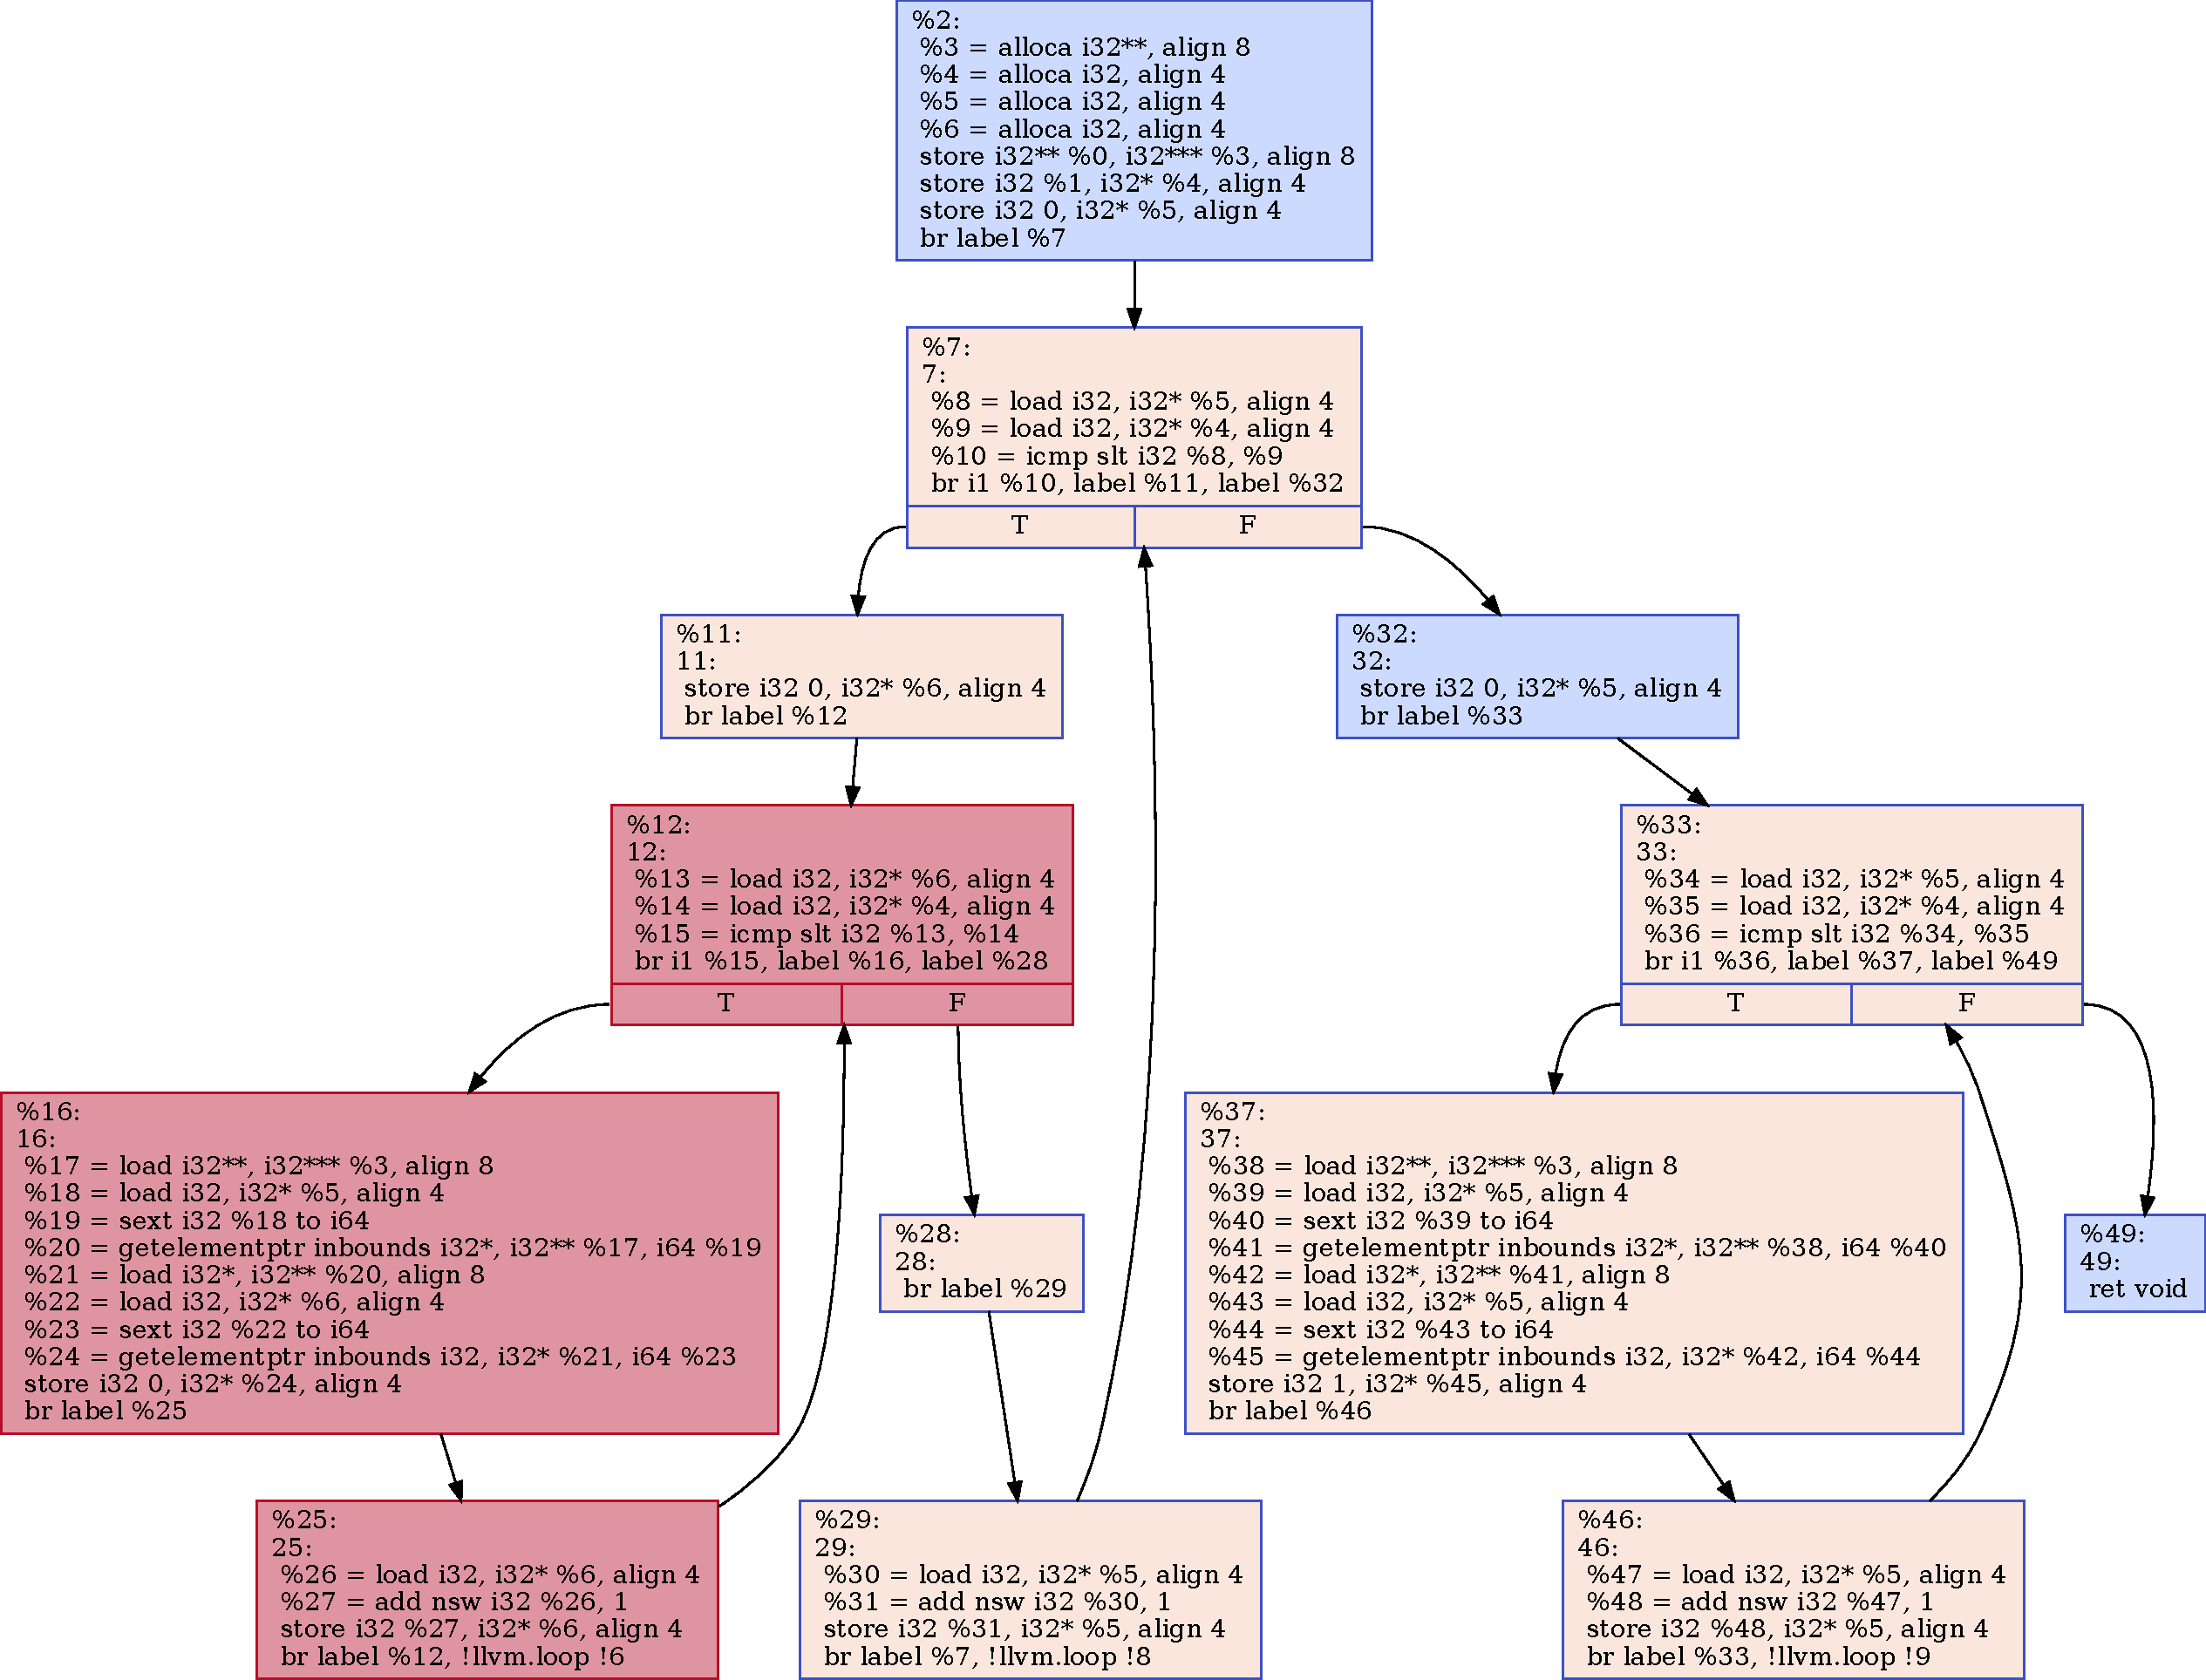
\includegraphics[width=\textwidth]{images/cfg.pdf}
    \caption{CFG's example}
    \label{fig:cfg_foo}
\end{figure}